%实验报告-衍射实验

\documentclass[a4paper]{article}%A4纸,文档类型为论文

%宏包
%文字设置
\usepackage[UTF8]{ctex}%处理中文
\usepackage{xeCJK}%处理中文
\usepackage{fontspec,xunicode,xltxtra}%字体设置
%文档&排版设置
\usepackage{titlesec}%自定义章节标题样式
\usepackage{multicol}%分栏
\usepackage{hyperref}%超链接设置\daleth 
\usepackage{multirow,makecell}%制作复杂表格
\usepackage{booktabs}%画三线表要用
\usepackage{float}%图片、表格等位置浮动排版
\usepackage{indentfirst}%首行缩进
\usepackage{graphicx,subfigure}%图片插入
\usepackage{listings}%代码高亮
\usepackage{xcolor}
\usepackage{appendix}%附录
\usepackage{fancyhdr}%页眉页脚
\usepackage{geometry}%页边距
\usepackage{caption}
%数学
\usepackage{amsmath,amssymb}%公式
\usepackage{amsfonts,mathrsfs,txfonts}%数学字体
\usepackage{array}%矩阵
\usepackage{gensymb}%角度单位“度”的命令:\degree

\geometry{a4paper,scale=0.8}%设置了纸张为a4,并且版心占页面长度的比例为80%;scale也可以改为ratio,表示版面边距占页面长度的比例.
\hypersetup{colorlinks=true,linkcolor=black,citecolor=black}%去掉目录等超链接所带的红框,并让参考文献的引用颜色为黑色
\setlength{\parindent}{2em}%首行缩进2字符
\lstset{
    columns=fixed,
    numbers=left, % 在左侧显示行号
    numberstyle=\footnotesize\color{darkgray},% 设定行号格式
    backgroundcolor=\color[RGB]{245,245,244},% 设定背景颜色
    keywordstyle=\color[RGB]{40,40,255},% 设定关键字颜色
    numberstyle=\color[RGB]{0,192,192},%行号数字样式
    commentstyle=\it\color[RGB]{0,96,96},% 设置代码注释的格式
    stringstyle=\rmfamily\slshape\color[RGB]{128,0,0},% 设置字符串格式
}
\pagestyle{fancy}%页眉页脚
\fancyhead{}%清空页眉
\fancyhead[C]{\emph{实验报告:衍射实验}}


\newcommand{\kaiti}{\CJKfamily{STKaiti}} % 楷体:\kaiti或\emph
\newcommand{\fs}{\CJKfamily{STFangsong}} % 仿宋:\fs或\fangsong
%黑体:\heiti

\newcommand{\suo}{\indent}%缩进2个字符

\title{\heiti{实验报告}}%标题
\author{{\emph{李佩哲}}}
\date{\emph{\small\today}}

\begin{document}
\begin{center}
\center{\bf{\LARGE{实验报告}\\\large{衍射实验}}}\\
\emph{李佩哲~~~PB21051049~~~\\\today}
\end{center}

\section{实验目的}
观察不同光学元件的夫琅禾费衍射图样,寻找规律并计算单双缝的缝宽.

\section{原理}
单缝的k级暗条纹到中央主极大的距离与单缝缝宽$a$关系为$$\frac{k\lambda}{a}=\frac{x_k}{L}$$
双峰的条纹宽度与双缝中心间距$d$关系为$$x_k=\frac{L}{d}\lambda$$
由此可计算单缝缝宽$a$与双缝中心间距$d$.

\section{实验仪器}
光学导轨,He-Ne激光器,衰减片,衍射元件,CCD等.

\section{测量记录}
原始数据见附件.\\整理如下
\\\suo $L=33.00~$cm,$\lambda=632.8~$nm.
\begin{table}[H]
    \begin{minipage}{0.18\linewidth}
        \centering
        \begin{tabular}{cc}
            \toprule
            $k$ & 坐标/mm\\
            \midrule
            +4&21.523\\
            +3&19.430\\
            +2&17.352\\
            +1&15.078\\
            0&13.968\\
            -1&10.742\\
            -2&8.563\\
            -3&6.557\\
            -4&4.366\\
            \bottomrule
        \end{tabular}
        \caption{100$~\mu$m单缝}\label{1}
    \end{minipage}
    \begin{minipage}{0.18\linewidth}  
        \centering
        \begin{tabular}{cc} 
            \toprule
            $k$ & 坐标/mm\\
            \midrule
            +4&17.198\\
            +3&16.121\\
            +2&15.024\\
            +1&13.987\\
            0&12.926\\
            -1&11.802\\
            -2&10.788\\
            -3&9.669\\
            -4&8.669\\
            \bottomrule
        \end{tabular}
        \caption{200$~\mu$m单缝}
    \end{minipage}
    \begin{minipage}{0.18\linewidth}  
        \centering
        \begin{tabular}{cc} 
            \toprule
            $k$ & 坐标/mm\\
            \midrule
            +4&15.684\\
            +3&14.977\\
            +2&14.298\\
            +1&13.585\\
            0&12.840\\
            -1&12.095\\
            -2&11.918\\
            -3&10.698\\
            -4&9.978\\
            \bottomrule
        \end{tabular}
        \caption{300$~\mu$m单缝}
    \end{minipage}
    \begin{minipage}{0.14\linewidth}
        \centering
        \begin{tabular}{c}
            \toprule
            坐标/mm\\
            \midrule
            18.635\\
            16.972\\
            15.949\\
            14.852\\
            12.406\\
            10.475\\
            8.938\\
            7.868\\
            \bottomrule
        \end{tabular}
        \caption{100$~\mu$m双缝}
    \end{minipage}
    \begin{minipage}{0.13\linewidth}  
        \centering
        \begin{tabular}{c} 
            \toprule
            坐标/mm\\
            \midrule
            17.262\\
            16.258\\
            15.572\\
            14.854\\
            12.975\\
            11.727\\
            10.613\\
            9.855\\
            \bottomrule
        \end{tabular}
        \caption{150$~\mu$m双缝}
    \end{minipage}
    \begin{minipage}{0.13\linewidth}  
        \centering
        \begin{tabular}{ccc} 
            \toprule
            坐标/mm\\
            \midrule
            15.305\\
            14.286\\
            13.239\\
            12.149\\
            11.150\\
            10.255\\
            9.728\\
            7.795\\
            \bottomrule
        \end{tabular}
        \caption{190$~\mu$m双缝}\label{2}
    \end{minipage}
\end{table}

\section{分析与讨论}
\subsection{图样特点}
单缝:中央有一条亮条纹,其余亮条纹亮度、宽度向两侧依次递减.

双缝:各条纹亮度、宽度基本不变,但偶尔会出现缺级,出现缺级处满足的条件为$\frac{n}{k}=\frac{d}{a}$.

小孔:中心有一个大的亮斑,而后其余亮条纹呈环状,亮度向外侧依次递减.

\subsection{变化规律}
单缝:随着缝宽增加,条纹宽度、间距减小.

双缝:随着双缝中心间距增加,条纹宽度、间距减小.

小孔:随着孔径增加,条纹宽度、间距减小.

\subsection{单缝缝宽与双缝中心间距的计算}
选取表\ref{1}与表\ref{2}为例,计算各自的$x_k$如下
\begin{table}[H]
    \begin{minipage}{0.25\linewidth}
        \centering
        \begin{tabular}{cc}
            \toprule
            $k$ &$x_k$/mm\\
            \midrule
            +4&7.555\\
            +3&5.462\\
            +2&3.384\\
            +1&1.110\\
            0&0.000\\
            -1&-3.226\\
            -2&-5.405\\
            -3&-7.411\\
            -4&-9.602\\
            \bottomrule
        \end{tabular}
        \caption{100$~\mu$m单缝}\label{3}
    \end{minipage}
    \begin{minipage}{0.25\linewidth}
        \centering
        \begin{tabular}{c}
            \toprule
            $x_k$/mm\\
            \midrule
            1.019\\
            1.047\\
            1.090\\
            0.999\\
            0.895(舍)\\
            0.527(舍)\\
            1.933(舍)\\
            \bottomrule
        \end{tabular}
        \caption{190$~\mu$m双缝}\label{4}
    \end{minipage}
    \begin{minipage}{0.5\linewidth}
        \centering
        \begin{figure}[H]
            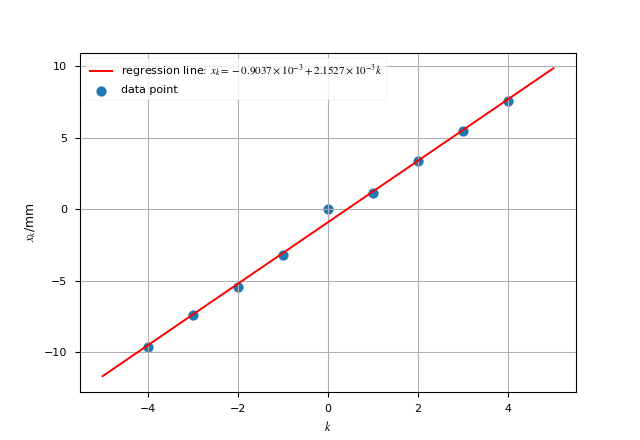
\includegraphics[scale=0.5]{Figure.png}
            \caption{$k-x_k$图}\label{0}
        \end{figure}
    \end{minipage}
\end{table}
对表\ref{3}作$k-x_k$图如图\ref{0},得$\frac{\lambda L}{a}=2.1527\pm 0.01255~$mm,从而$a\approx 97.01\pm 0.5656~\mu$m.误差为2.990\%.

对表\ref{4}求$\overline{x_k}=1.010\pm 0.05446~$mm$=\lambda \frac{L}{d}$,从而$d=201.0\pm 10.85~\mu$m.误差为5.789\%.

\subsection{思考题}
当光通过小孔时的图案为中心有一个大的亮斑,而后其余亮条纹呈环状,亮度向外侧依次递减.当小孔直径较大而不足以发生明显衍射时,光屏上的像为光源倒立的形状.

白光照射到单缝时会发生色散,不同波长的光各自发生衍射,体现为中央亮条纹为白色,两侧的条纹为叠加的彩色.如下图
\begin{figure}[H]
    \centering
    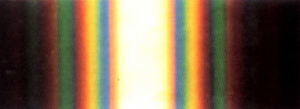
\includegraphics[scale=.4]{1.png}
\end{figure}

\end{document}